% ========================================================
% EdgeGuard-IoT | Beamer Pitch Deck
% Tema: Minimalista Académico Oscuro (pdflatex compatible)
% Autora: Carmen Nieves Apaza Condori
% EPIS — Universidad Nacional del Altiplano de Puno, 2026
% Compilar: pdflatex -> pdflatex (2 pasadas)
% ========================================================
\documentclass[aspectratio=169, 10pt]{beamer}

% ----- Paquetes Base ----------------------------------
\usepackage[utf8]{inputenc}
\usepackage[T1]{fontenc}
\usepackage[spanish]{babel}
\usepackage{lmodern}

% ----- Paquetes Adicionales ---------------------------
\usepackage{amsmath, amssymb}
\usepackage{graphicx}
\usepackage{booktabs}
\usepackage{colortbl}
\usepackage{microtype}
\usepackage{tikz}
\usetikzlibrary{positioning, arrows.meta, shapes.geometric, fit, calc, backgrounds}

% =====================================================
% PALETA DE COLORES MINIMALISTA OSCURA
% =====================================================
\definecolor{bgdark}{HTML}{0B0F1A}
\definecolor{bgpanel}{HTML}{111827}
\definecolor{bgcard}{HTML}{1A2235}
\definecolor{cyanneon}{HTML}{00BCD4}
\definecolor{bluesoft}{HTML}{4A90D9}
\definecolor{goldacc}{HTML}{C9A84C}
\definecolor{redsoft}{HTML}{E05260}
\definecolor{greensoft}{HTML}{38A169}
\definecolor{textmain}{HTML}{EEF2FF}
\definecolor{textmuted}{HTML}{64748B}
\definecolor{bordercol}{HTML}{1E2D4A}

% =====================================================
% CONFIGURACIÓN BEAMER — TEMA MINIMALISTA PERSONALIZADO
% =====================================================
\usetheme{default}
\usecolortheme{default}

% Background
\setbeamercolor{background canvas}{bg=bgdark}
\setbeamercolor{normal text}{fg=textmain, bg=bgdark}

% Frame title
\setbeamercolor{frametitle}{fg=textmain, bg=bgpanel}
\setbeamerfont{frametitle}{size=\large, series=\bfseries}
\setbeamertemplate{frametitle}{
  \vspace*{0.18cm}
  \insertframetitle
  \vspace*{0.06cm}
  \par\noindent{\color{cyanneon}\rule{\textwidth}{0.6pt}}
}

% Items
\setbeamercolor{itemize item}{fg=cyanneon}
\setbeamercolor{itemize subitem}{fg=bluesoft}
\setbeamercolor{enumerate item}{fg=cyanneon}
\setbeamertemplate{itemize item}{\textcolor{cyanneon}{$\bullet$}}
\setbeamertemplate{itemize subitem}{\textcolor{bluesoft}{$\circ$}}
\setbeamertemplate{enumerate item}{\textcolor{cyanneon}{\insertenumlabel.}}

% Block
\setbeamercolor{block title}{fg=cyanneon, bg=bgcard}
\setbeamercolor{block body}{fg=textmain, bg=bgcard}
\setbeamerfont{block title}{series=\bfseries, size=\small}
\setbeamerfont{block body}{size=\small}
\setbeamertemplate{blocks}[rounded][shadow=false]

% Navigation symbols: remove
\setbeamertemplate{navigation symbols}{}

% Footer minimalista
\setbeamertemplate{footline}{
  \begin{beamercolorbox}[ht=0.4cm, dp=0.2cm, leftskip=0.3cm, rightskip=0.3cm]{normal text}
    \color{textmuted}\tiny
    Carmen Nieves Apaza Condori \hfill
    EdgeGuard-IoT $\cdot$ EPIS -- UNAP 2026 \hfill
    \insertframenumber{}/\inserttotalframenumber
  \end{beamercolorbox}
}

% Alertas
\setbeamercolor{alerted text}{fg=redsoft}

% =====================================================
% METADATA
% =====================================================
\title{\textbf{EdgeGuard-IoT}}
\subtitle{Sistema Adaptativo de Detección de Botnets Multiclase\\
          mediante VAE-MLP INT8 y SHAP XAI en el Borde}
\author{Carmen Nieves Apaza Condori}
\institute{EPIS --- Universidad Nacional del Altiplano de Puno}
\date{2026}

% =====================================================
\begin{document}
% =====================================================

% ----- PORTADA ----------------------------------------
{
\setbeamertemplate{footline}{}
\setbeamertemplate{frametitle}{}
\begin{frame}[plain]
  \begin{tikzpicture}[remember picture, overlay]
    % Línea superior decorativa
    \fill[cyanneon] (current page.north west) rectangle +(\paperwidth, -3pt);
    % Panel lateral izquierdo
    \fill[bgpanel] (current page.north west) rectangle +(0.08\paperwidth, -\paperheight);
    % Barra decorativa izquierda
    \fill[cyanneon] (current page.north west) rectangle +(3pt, -\paperheight);
  \end{tikzpicture}

  \hspace{0.1\textwidth}%
  \begin{minipage}{0.85\textwidth}
    \vspace{1.4cm}
    {\color{textmuted}\footnotesize Tópicos en Ciberseguridad II \quad $\cdot$ \quad
     Docente: Ing. Ticona Yanqui Fidel Ernesto}

    \vspace{0.4cm}
    {\color{cyanneon}\LARGE\bfseries EdgeGuard-IoT}

    \vspace{0.3cm}
    {\color{textmain}\large Sistema Adaptativo de Detección de\\Botnets Multiclase mediante VAE-MLP INT8 y SHAP XAI}

    \vspace{0.5cm}
    {\color{textmuted}\rule{0.75\textwidth}{0.4pt}}

    \vspace{0.4cm}
    \begin{tabular}{lll}
      {\color{cyanneon}\large\bfseries 77.18\%} &
      {\color{goldacc}\large\bfseries 21.67 KB} &
      {\color{bluesoft}\large\bfseries 3.25 $\mu$s} \\[2pt]
      {\color{textmuted}\footnotesize Accuracy Nube} &
      {\color{textmuted}\footnotesize Footprint ONNX INT8} &
      {\color{textmuted}\footnotesize Latencia Borde}
    \end{tabular}

    \vspace{0.6cm}
    {\color{textmuted}\small Carmen Nieves Apaza Condori}\\
    {\color{textmuted}\small EPIS --- Universidad Nacional del Altiplano de Puno}\\
    {\color{textmuted}\small 2026}
  \end{minipage}
\end{frame}
}

% ----- AGENDA -----------------------------------------
\begin{frame}{Agenda de la Presentación}
  \begin{columns}[T]
    \begin{column}{0.48\textwidth}
      \begin{enumerate}\small
        \item[\textcolor{cyanneon}{01}] Motivación y Problema de Investigación
        \item[\textcolor{cyanneon}{02}] Objetivos e Hipótesis
        \item[\textcolor{cyanneon}{03}] Arquitectura del Sistema EdgeGuard-IoT
        \item[\textcolor{cyanneon}{04}] Dataset y Metodología MLOps
      \end{enumerate}
    \end{column}
    \begin{column}{0.48\textwidth}
      \begin{enumerate}\small
        \item[\textcolor{goldacc}{05}] Resultados: Selección de Características
        \item[\textcolor{goldacc}{06}] Resultados: Entrenamiento y Evaluación
        \item[\textcolor{goldacc}{07}] Benchmark del Estado del Arte
        \item[\textcolor{goldacc}{08}] Interpretabilidad SHAP XAI
        \item[\textcolor{cyanneon}{09}] Despliegue en Producción
        \item[\textcolor{cyanneon}{10}] Conclusiones y Trabajo Futuro
      \end{enumerate}
    \end{column}
  \end{columns}
\end{frame}

% =====================================================
% 01 - PROBLEMA
% =====================================================
\begin{frame}{01 \quad El Trilema de la Ciberseguridad en la IoT}
  \begin{columns}[T, onlytextwidth]
    \begin{column}{0.32\textwidth}
      \begin{block}{\textcolor{redsoft}{Latencia en la Nube}}
        \small Los IDS centralizados requieren transmitir flujos masivos de paquetes.
        La latencia de transporte ($>200$ ms) impide la respuesta en tiempo real
        ante botnets de propagación relámpago.
      \end{block}
    \end{column}
    \begin{column}{0.32\textwidth}
      \begin{block}{\textcolor{goldacc}{Memoria Restringida}}
        \small Los microcontroladores empotrados (ARM Cortex-M, ESP32) poseen
        $\leq 512$ KB de RAM. Un Random Forest estándar supera los 50 MB de
        footprint en disco.
      \end{block}
    \end{column}
    \begin{column}{0.32\textwidth}
      \begin{block}{\textcolor{bluesoft}{Opacidad Algorítmica}}
        \small Las soluciones de DL pesadas operan como \textit{cajas negras},
        impidiendo auditorías forenses en tiempo real en Centros de Operaciones
        de Ciberseguridad (SOC).
      \end{block}
    \end{column}
  \end{columns}

  \vspace{0.5cm}
  \begin{center}
    \begin{tikzpicture}
      \node[draw=cyanneon, fill=bgcard, rounded corners=4pt, inner sep=8pt,
            text width=0.78\textwidth, align=center, text=textmain, font=\small]{
        \textcolor{cyanneon}{\textbf{Pregunta central:}} ¿Cómo desplegar un IDS multiclase
        que sea \textit{ultraligero} ($\leq 30$ KB), \textit{preciso} ($>75\%$) y
        \textit{explicable} (SHAP XAI) simultáneamente sobre hardware periférico?
      };
    \end{tikzpicture}
  \end{center}
\end{frame}

% =====================================================
% 02 - OBJETIVOS
% =====================================================
\begin{frame}{02 \quad Objetivos e Hipótesis de Investigación}
  \begin{columns}[T]
    \begin{column}{0.54\textwidth}
      \textbf{Objetivo General}\\[4pt]
      \textcolor{textmuted}{\small Desarrollar y evaluar EdgeGuard-IoT: arquitectura
      híbrida Borde-Nube con VAE-MLP INT8 en el borde, Stacking Ensemble
      LightGBM en la nube y SHAP XAI, sobre el benchmark CIC-IoT-2023.}

      \vspace{10pt}
      \textbf{Hipótesis Alternativa $H_1$}\\[4pt]
      \textcolor{textmuted}{\small La arquitectura propuesta logra inferencia ultra-rápida
      en el borde ($\leq 5\,\mu\text{s}$, footprint $\leq 30$ KB) y una precisión consolidada
      $> 75\%$ de Accuracy en la nube con interpretabilidad SHAP XAI.}
    \end{column}

    \begin{column}{0.43\textwidth}
      \begin{block}{Objetivos Específicos}
        \begin{enumerate}\footnotesize
          \item Preprocesamiento y selección estadística de características\\
                (ANOVA F-Test, Mutual Information, Gini).
          \item Diseño, entrenamiento y cuantificación ONNX INT8 del VAE-MLP.
          \item Construcción del Stacking Ensemble y evaluación frente
                al estado del arte con SHAP XAI.
        \end{enumerate}
      \end{block}
    \end{column}
  \end{columns}
\end{frame}

% =====================================================
% 03 - ARQUITECTURA
% =====================================================
\begin{frame}{03 \quad Arquitectura Híbrida Adaptativa Borde-Nube}
  \begin{center}
  \resizebox{0.92\textwidth}{!}{%
  \begin{tikzpicture}[
    node distance=0.8cm and 1.2cm,
    box/.style={rectangle, draw=bordercol, fill=bgcard, rounded corners=3pt,
                text width=2.2cm, align=center, minimum height=0.9cm,
                font=\small\bfseries, text=textmain},
    cyanbox/.style={box, draw=cyanneon, text=cyanneon, fill=bgdark},
    goldbox/.style={box, draw=goldacc, text=goldacc, fill=bgdark, text width=2.4cm},
    arrow/.style={->, >=Stealth, thick, color=cyanneon!70},
    lbl/.style={font=\footnotesize\bfseries, text=textmuted}
  ]
    \node[box, draw=bluesoft, text=bluesoft] (inp) {Tráfico IoT\\39 Features};

    \node[cyanbox, right=1.1cm of inp] (vae)
          {VAE-MLP\\INT8 ONNX\\[2pt]{\tiny 21.67 KB | 3.25 $\mu$s}};

    \node[box, right=1.2cm of vae, yshift=+1.0cm] (xgb) {XGBoost};
    \node[box, right=1.2cm of vae] (rf) {Random\\Forest};
    \node[box, right=1.2cm of vae, yshift=-1.0cm] (lgb) {LightGBM};

    \node[goldbox, right=1.3cm of rf]
          (meta) {Meta-Learner\\LightGBM\\[2pt]{\tiny $\mathbf{M} \in \mathbb{R}^{32}$}};

    \node[box, right=1.1cm of meta, draw=greensoft, text=greensoft, fill=bgdark]
          (out) {Veredicto\\Multiclase\\+ SHAP XAI};

    \node[lbl, above=0.25cm of vae]  {\textbf{Capa 1: Borde}};
    \node[lbl, above=0.25cm of xgb] {\textbf{Capa 2: Nube — Nivel 0}};
    \node[lbl, above=0.25cm of meta] {\textbf{Nivel 1: Meta-Learner}};

    \draw[arrow] (inp) -- (vae);
    \draw[arrow] (vae) -- (xgb);
    \draw[arrow] (vae) -- (rf);
    \draw[arrow] (vae) -- (lgb);
    \draw[arrow] (xgb) -- (meta);
    \draw[arrow] (rf)  -- (meta);
    \draw[arrow] (lgb) -- (meta);
    \draw[arrow] (meta) -- (out);

    \begin{pgfonlayer}{background}
      \node[draw=cyanneon, fill=cyanneon!5, dashed, rounded corners=4pt,
            fit=(vae), inner sep=6pt] {};
      \node[draw=goldacc, fill=goldacc!5, dashed, rounded corners=4pt,
            fit=(xgb)(rf)(lgb), inner sep=6pt] {};
    \end{pgfonlayer}
  \end{tikzpicture}}
  \end{center}

  \vspace{0.15cm}
  \begin{columns}
    \column{0.5\textwidth}\small
    \textcolor{textmuted}{El \textcolor{cyanneon}{\textbf{VAE-MLP INT8}} opera autónomamente
    con $3.25\,\mu\text{s}$ de latencia y solo $21.67$ KB de footprint.}
    \column{0.5\textwidth}\small
    \textcolor{textmuted}{El \textcolor{goldacc}{\textbf{Stacking Ensemble}} consolida
    la predicción final con \textbf{77.18\%} de Accuracy.}
  \end{columns}
\end{frame}

% =====================================================
% 04 - DATASET Y METODOLOGÍA
% =====================================================
\begin{frame}{04 \quad Dataset CIC-IoT-2023 y Pipeline MLOps}
  \begin{columns}[T]
    \begin{column}{0.47\textwidth}
      \begin{block}{Dataset CIC-IoT-2023}
        \begin{itemize}\small
          \item \textbf{186,321} muestras balanceadas estratificadamente.
          \item \textbf{39} características tabulares de flujo de red.
          \item \textbf{8 clases:} Benigno + 7 tipos de ataque botnet.
          \item Partición: 70\% Train / 15\% Val / 15\% Test.
        \end{itemize}
      \end{block}

      \vspace{5pt}
      \begin{block}{Ataques Evaluados}
        \footnotesize
        DDoS-UDP $\cdot$ DDoS-TCP SYN $\cdot$ DDoS-ICMP $\cdot$ DoS\\
        Mirai Botnet $\cdot$ Reconnaissance $\cdot$ Spoofing ARP\\
        Brute Force $\cdot$ Web-Based Attacks
      \end{block}
    \end{column}

    \begin{column}{0.50\textwidth}
      \textbf{Pipeline de 5 Fases MLOps:}\\[6pt]
      \begin{enumerate}\small
        \item[\textcolor{cyanneon}{1.}] \textbf{Preprocesamiento:} Ingestión por fragmentos,
              limpieza estricta y normalización MinMaxScaler.
        \item[\textcolor{cyanneon}{2.}] \textbf{Selección estadística:} ANOVA F-Test,
              Mutual Info y Gini $\Rightarrow$ Top-15 características.
        \item[\textcolor{cyanneon}{3.}] \textbf{Entrenamiento:} VAE-MLP en GPU CUDA,
              40 épocas, Class-Weighted Loss + CosineAnnealingLR.
        \item[\textcolor{cyanneon}{4.}] \textbf{Cuantificación:} Export ONNX FP32
              $\rightarrow$ INT8 dando $21.67$ KB.
        \item[\textcolor{goldacc}{5.}] \textbf{Evaluación:} Stacking + 5-Fold CV + SHAP XAI.
      \end{enumerate}
    \end{column}
  \end{columns}
\end{frame}

% =====================================================
% 05 - SELECCIÓN DE CARACTERÍSTICAS
% =====================================================
\begin{frame}{05 \quad Selección Estadística de Características}
  \begin{columns}[T]
    \begin{column}{0.57\textwidth}
      \centering
      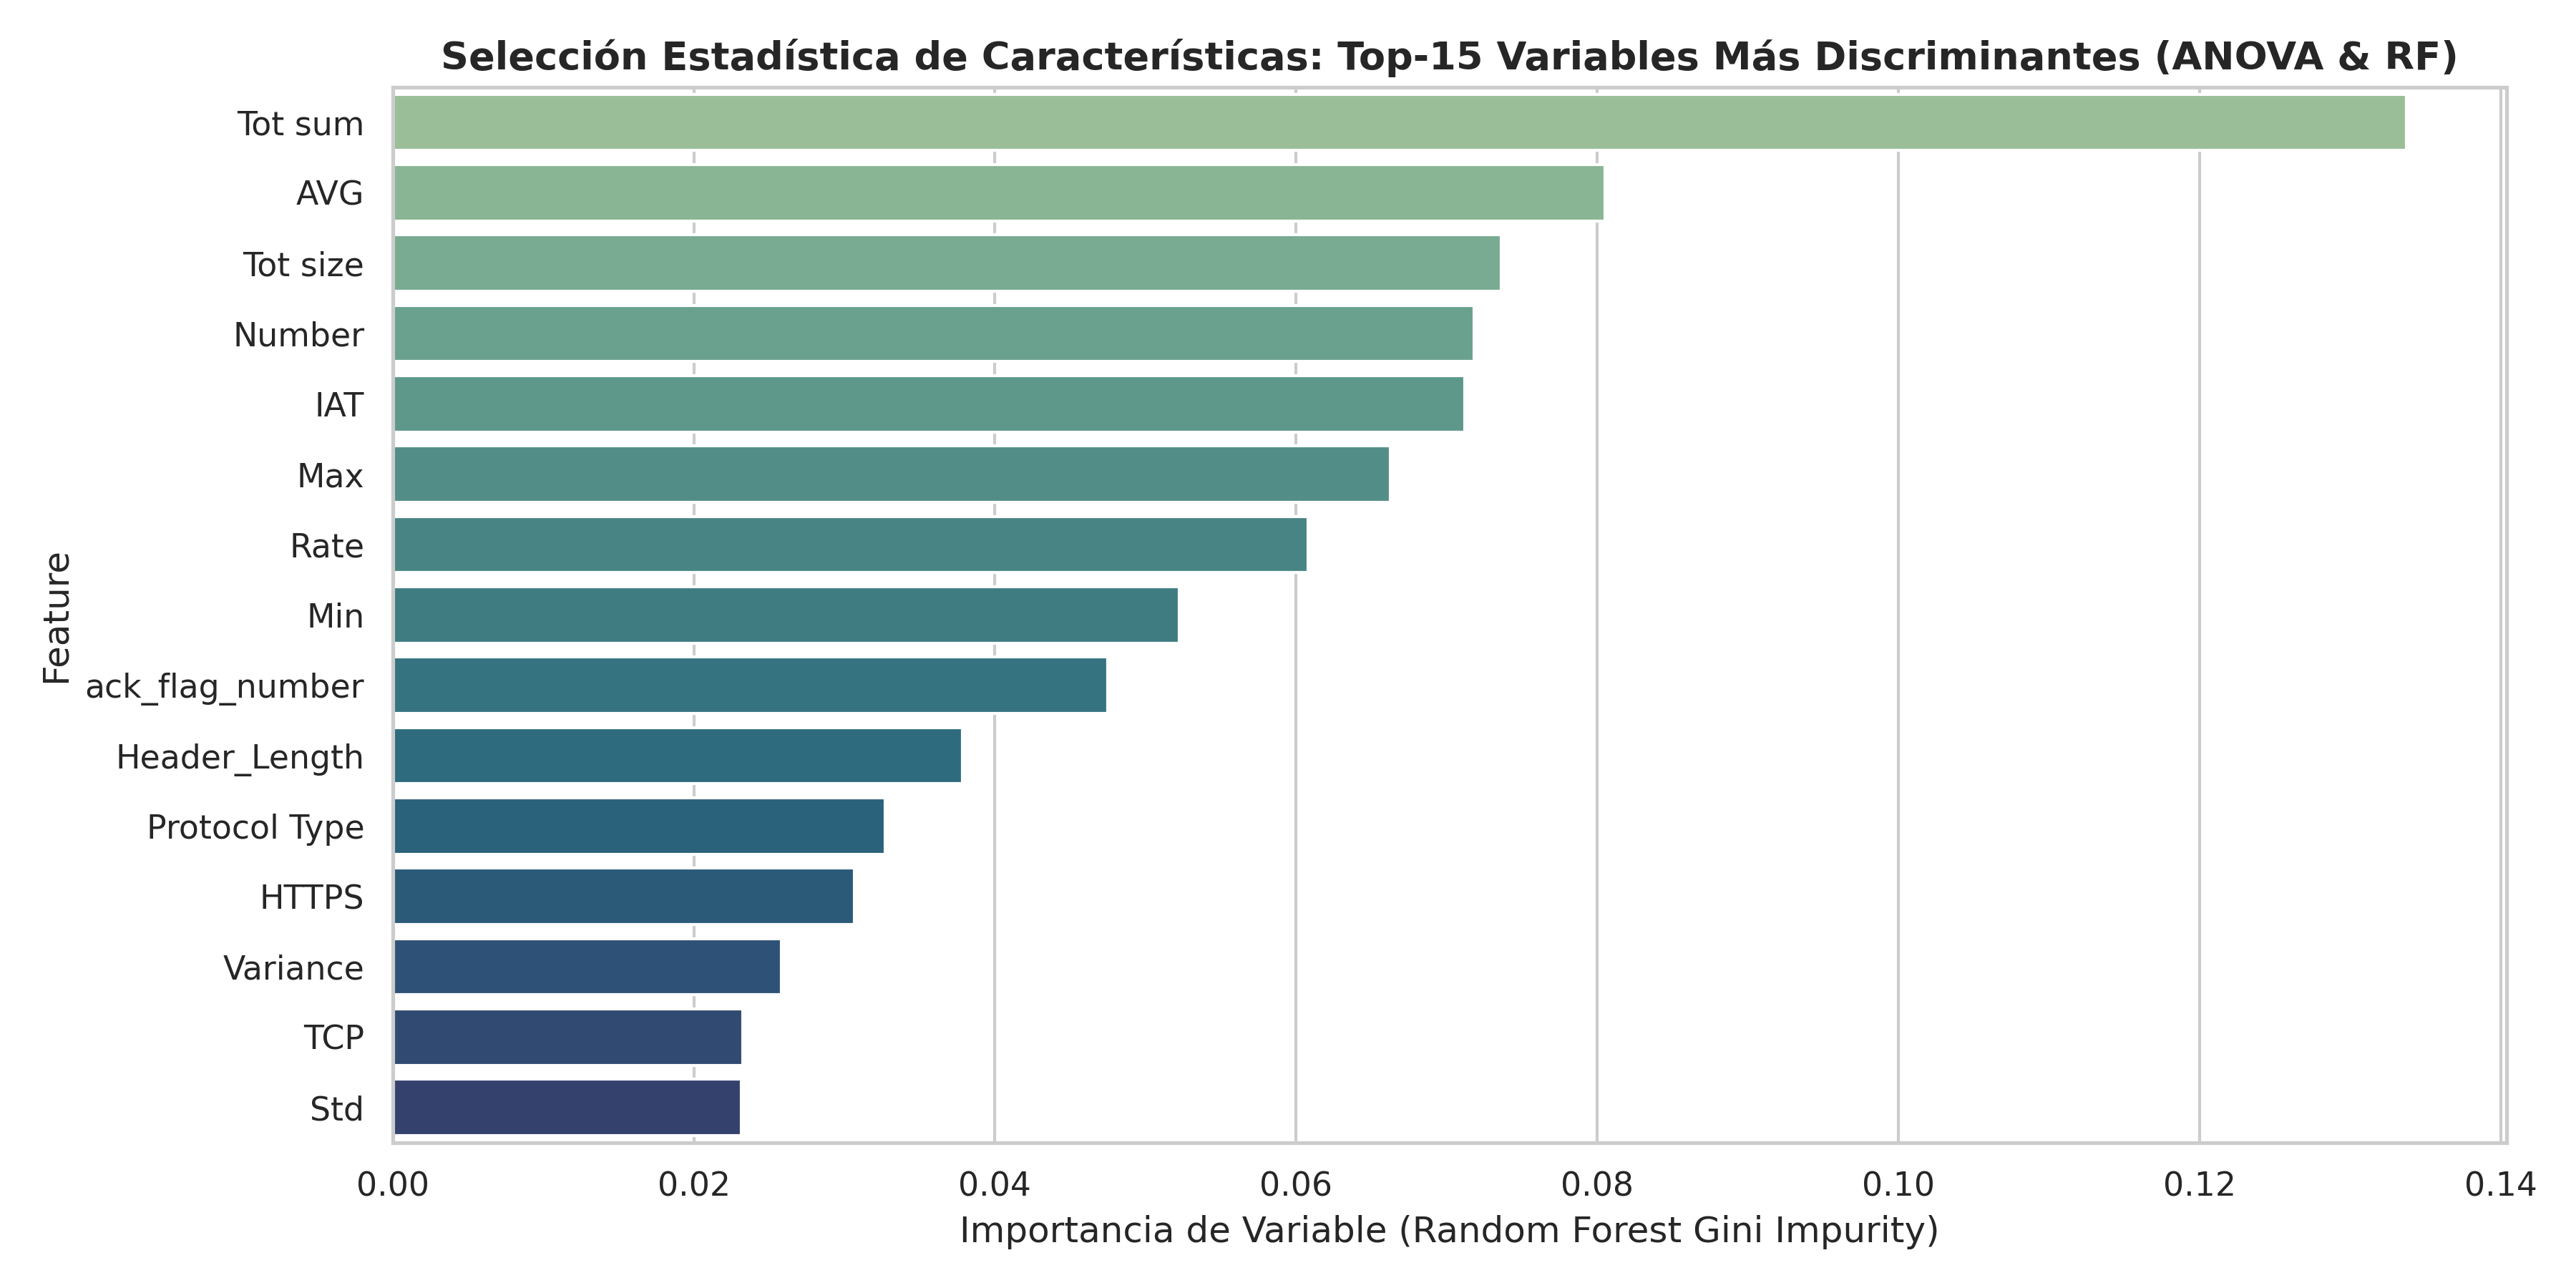
\includegraphics[width=\linewidth]{../../results/reports_and_plots/feature_selection_barplot.png}
      {\color{textmuted}\tiny Top-15 variables de red más discriminantes (ANOVA F-Test + Gini)}
    \end{column}
    \begin{column}{0.40\textwidth}
      \vspace{10pt}
      \textbf{Variables más relevantes:}\\[6pt]
      \begin{itemize}\small
        \item \texttt{Header\_Length}: firma principal de ataques con manipulación de cabeceras TCP/IP.
        \item \texttt{Rate} y \texttt{Tot sum}: atributos volumétricos para DDoS/DoS.
        \item \texttt{Protocol Type}: discrimina ICMP, UDP, ARP.
        \item \texttt{Telnet}: señal directa de infecciones Mirai.
      \end{itemize}

      \vspace{8pt}
      \textcolor{textmuted}{\footnotesize Los tres criterios (ANOVA, Mutual Information y Gini)
      coincidieron en la jerarquía de las 15 características seleccionadas, validando la
      consistencia estadística del conjunto de entrada.}
    \end{column}
  \end{columns}
\end{frame}

% =====================================================
% 06 - ENTRENAMIENTO Y MATRICES
% =====================================================
\begin{frame}{06 \quad Convergencia del VAE-MLP y Matrices de Confusión}
  \begin{columns}[T]
    \begin{column}{0.49\textwidth}
      \centering
      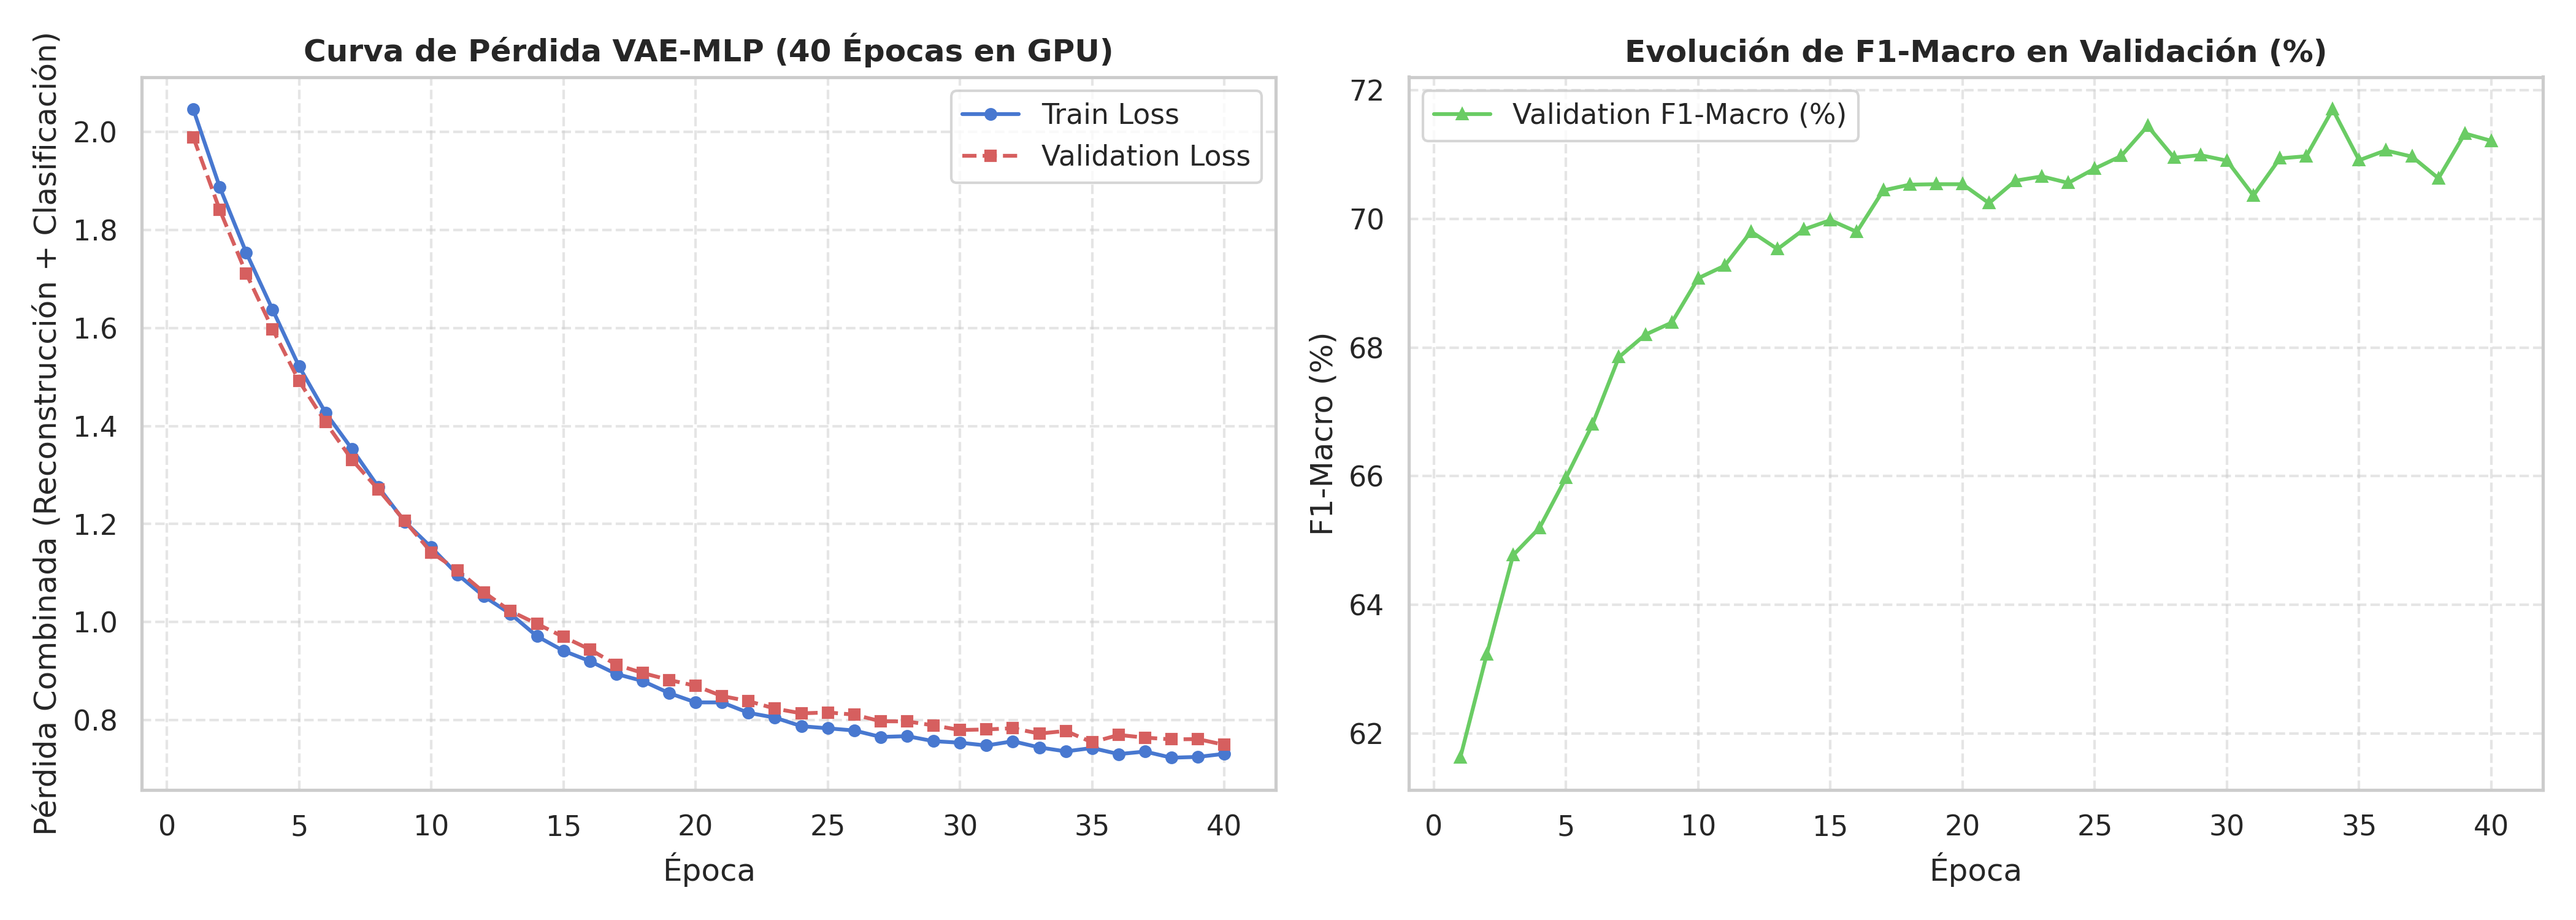
\includegraphics[width=\linewidth]{../../results/reports_and_plots/training_history_loss_f1.png}
      {\color{textmuted}\tiny Curvas de pérdida y F1-Macro durante las 40 épocas de entrenamiento}
    \end{column}
    \begin{column}{0.49\textwidth}
      \centering
      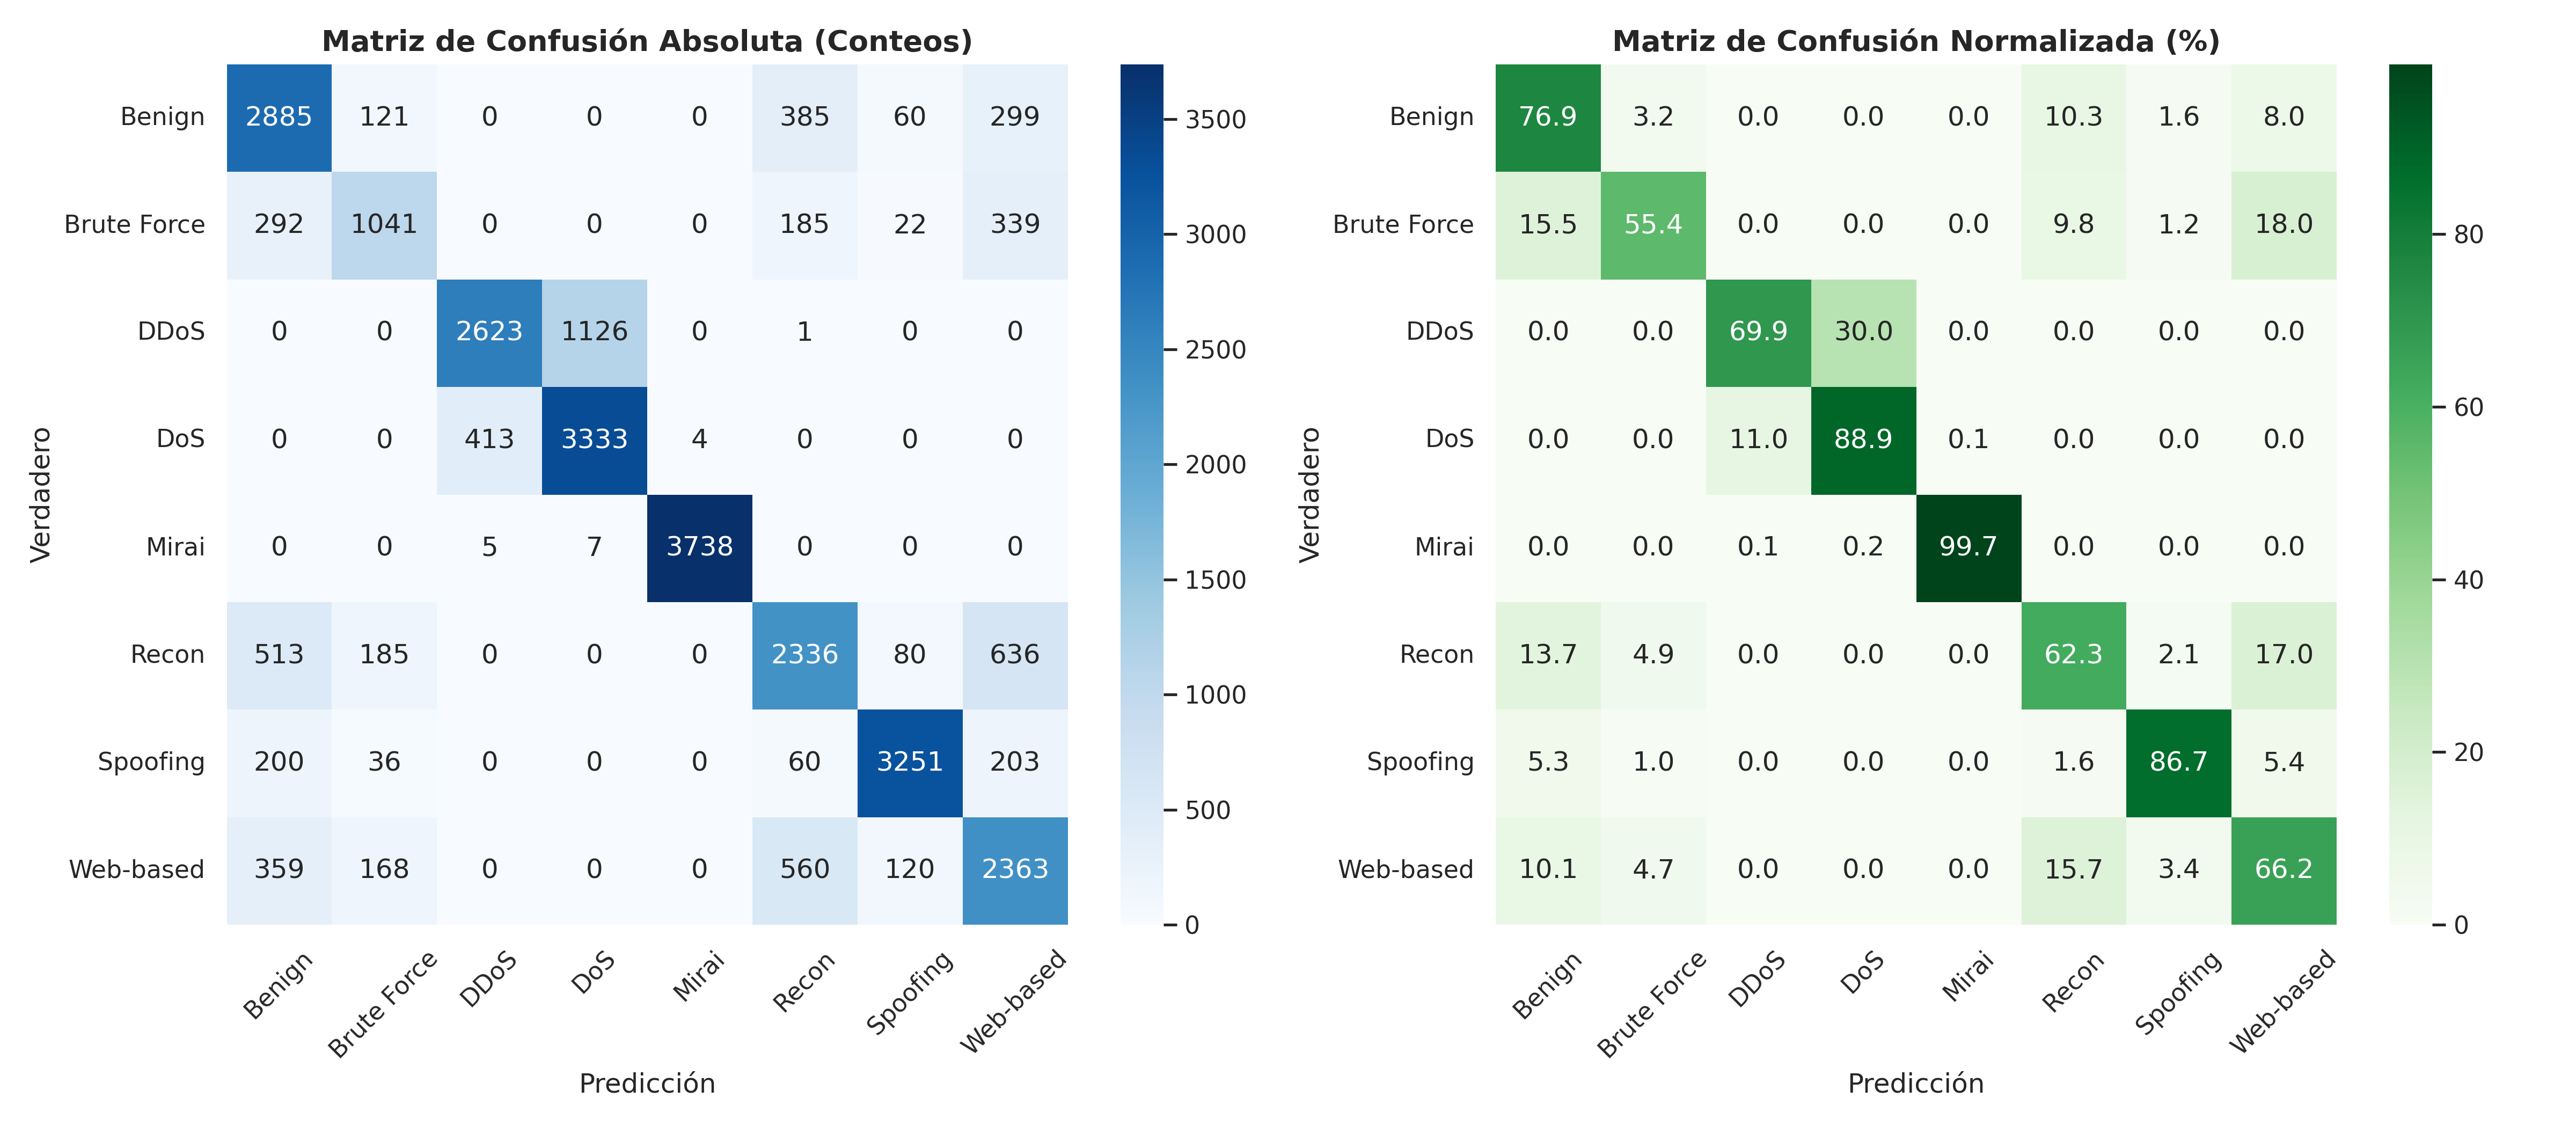
\includegraphics[width=\linewidth]{../../results/reports_and_plots/confusion_matrices_combined.png}
      {\color{textmuted}\tiny Matriz de Confusión Absoluta y Normalizada (\%) del Stacking Ensemble}
    \end{column}
  \end{columns}

  \vspace{0.2cm}
  \begin{columns}
    \column{0.5\textwidth}\footnotesize
    \textcolor{textmuted}{Convergencia estable a partir de la \textbf{época 25} sin sobreajuste apreciable.}
    \column{0.5\textwidth}\footnotesize
    \textcolor{textmuted}{\textbf{DDoS y Mirai:} $>96\%$ de detección correcta.
    \textbf{Web-Based:} mayor confusión con tráfico benigno.}
  \end{columns}
\end{frame}

% =====================================================
% 07 - BENCHMARK
% =====================================================
\begin{frame}{07 \quad Benchmark Comparativo del Estado del Arte}
  \begin{center}
  \small
  \begin{tabular}{lcccc}
    \toprule
    \textbf{Modelo}  &  \textbf{Accuracy (\%)}  &  \textbf{F1-Macro}  &  \textbf{Latencia ($\mu$s)}  &  \textbf{Tamaño (KB)} \\
    \midrule
    Reg. Logística   &  64.04  &  0.6233  &  185.27  &  15 \\
    Naive Bayes      &  56.87  &  0.5340  &  4.29    &  10 \\
    CNN-1D (DL)      &  61.91  &  0.5722  &  1.60    &  120 \\
    \midrule
    \rowcolor{cyanneon!15}
    \textbf{EdgeGuard VAE-MLP INT8} & \textbf{69.73} & \textbf{0.6853} & \textbf{3.25} & \textbf{21.67} \\
    \midrule
    Random Forest    &  76.61  &  0.7525  &  5.82    &  52{,}525 \\
    XGBoost          &  77.13  &  0.7585  &  2.68    &  4{,}021 \\
    LightGBM         &  77.73  &  0.7663  &  49.92   &  4{,}134 \\
    \midrule
    \rowcolor{goldacc!20}
    \textbf{$\star$ Stacking Ensemble} & \textbf{77.18} & \textbf{0.7604} & \textbf{2.45} & \textbf{1{,}400} \\
    \bottomrule
  \end{tabular}
  \end{center}

  \vspace{0.15cm}
  \textcolor{textmuted}{\footnotesize $\star$ Stacking = VAE-MLP + RF + XGB + LightGBM (Level-0) con Meta-Learner LightGBM (Level-1). Evaluado sobre \textbf{27{,}949} muestras de prueba independientes.}
\end{frame}

% =====================================================
% 08 - SHAP XAI
% =====================================================
\begin{frame}{08 \quad Interpretabilidad Forense con SHAP XAI}
  \begin{columns}[T]
    \begin{column}{0.51\textwidth}
      \centering
      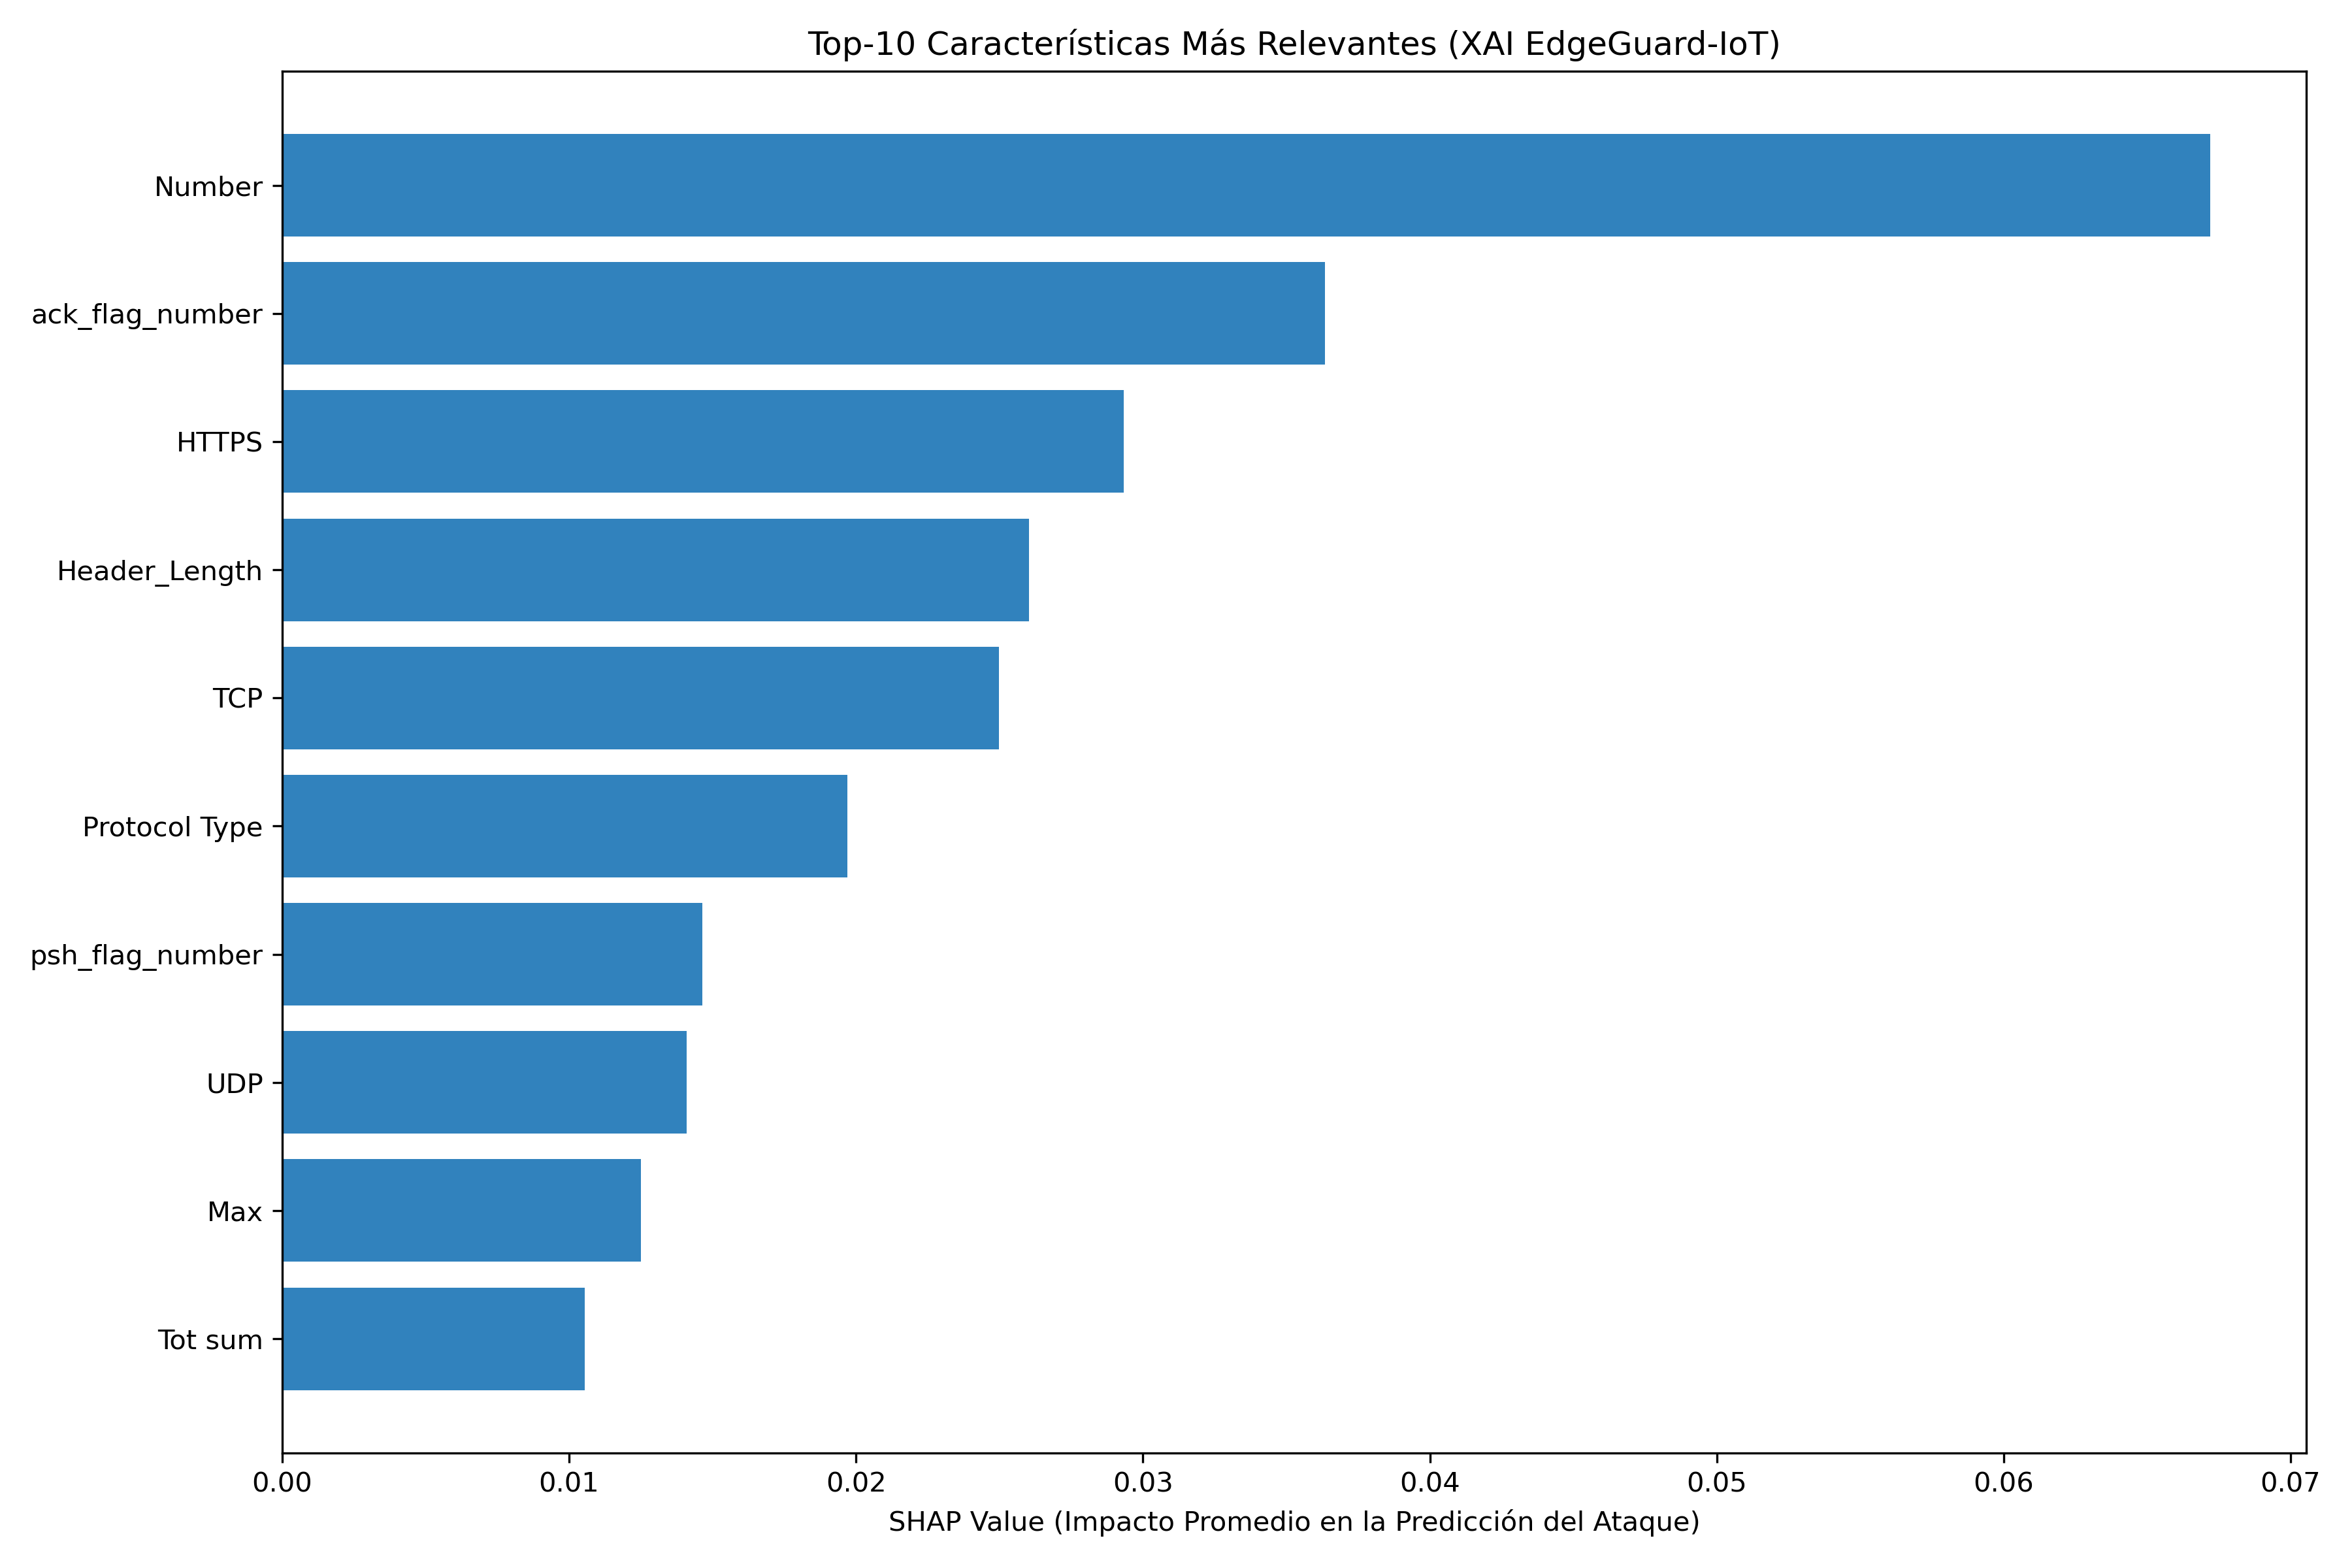
\includegraphics[width=0.96\linewidth]{../../results/reports_and_plots/shap_summary_plot.png}
      {\color{textmuted}\tiny Importancia SHAP por característica de red — Mayor valor = mayor impacto en predicción}
    \end{column}
    \begin{column}{0.45\textwidth}
      \vspace{6pt}
      \textbf{¿Por qué SHAP?}\\[5pt]
      \begin{itemize}\small
        \item Basado en la \textit{teoría de juegos cooperativos} de Shapley (1953).
        \item Garantiza \textbf{4 axiomas}: Eficiencia, Simetría, Jugador Nulo, Aditividad.
        \item Genera explicaciones \textit{locales} por cada flujo clasificado.
      \end{itemize}

      \vspace{8pt}
      \textbf{Integración MLOps en Producción:}\\[5pt]
      \begin{itemize}\small
        \item Endpoint FastAPI \texttt{/predict} $\Rightarrow$ retorna atribuciones SHAP.
        \item Dashboard Streamlit visualiza Top-3 factores en tiempo real.
      \end{itemize}
    \end{column}
  \end{columns}
\end{frame}

% =====================================================
% 09 - DESPLIEGUE
% =====================================================
\begin{frame}{09 \quad Despliegue MLOps y Microservicios en Producción}
  \begin{columns}[T]
    \begin{column}{0.48\textwidth}
      \begin{block}{Pila Tecnológica (Tech Stack)}
        \begin{itemize}\small
          \item \textbf{Edge:} ONNX Runtime INT8 en Python.
          \item \textbf{Backend API:} FastAPI + Uvicorn (Docker multi-etapa).
          \item \textbf{Frontend UI:} Streamlit Dashboard --- Tema Neón.
          \item \textbf{Cloud:} Render.com --- Contenedores en producción.
          \item \textbf{XAI:} SHAP integrado en el pipeline de inferencia.
          \item \textbf{Versión:} Git $+$ GitHub Actions CI/CD.
        \end{itemize}
      \end{block}
    \end{column}

    \begin{column}{0.48\textwidth}
      \begin{block}{Servicios en Vivo (Producción)}
        \small
        \textcolor{cyanneon}{\textbf{Dashboard Frontend Streamlit:}}\\
        \texttt{edgeguard-frontend.onrender.com}

        \vspace{6pt}
        \textcolor{cyanneon}{\textbf{API REST FastAPI Swagger:}}\\
        \texttt{edgeguard-backend.onrender.com/docs}

        \vspace{6pt}
        \textcolor{goldacc}{\textbf{Repositorio Oficial GitHub:}}\\
        \texttt{github.com/carmenNieves6478/EdgeGuard-{}-IoT}
      \end{block}
    \end{column}
  \end{columns}
\end{frame}

% =====================================================
% 10 - CONCLUSIONES
% =====================================================
\begin{frame}{10 \quad Conclusiones y Verificación de Hipótesis}
  \begin{columns}[T]
    \begin{column}{0.57\textwidth}
      \begin{enumerate}\small
        \item \textbf{Inferencia Edge ultraligera verificada:}\\
              VAE-MLP INT8 logra $3.25\,\mu\text{s}$ y $21.67$ KB,
              superando el umbral $H_1$ ($\leq 5\,\mu\text{s}$, $\leq 30$ KB).

        \item \textbf{Máxima precisión consolidada en la nube:}\\
              Stacking Ensemble alcanza $77.18\%$ Accuracy y F1-Macro $0.7604$.\\
              Estabilidad comprobada: $76.52\% \pm 0.18\%$ en 5-Fold CV.

        \item \textbf{Transparencia operacional SOC:}\\
              SHAP XAI emite atribuciones forenses locales por cada flujo
              clasificado en tiempo real.

        \vspace{4pt}
        \item[\textcolor{greensoft}{\checkmark}]
              \textbf{Se rechaza $H_0$ y se acepta $H_1$} con evidencia empírica
              sólida sobre $27{,}949$ muestras de prueba independientes.
      \end{enumerate}
    \end{column}

    \begin{column}{0.40\textwidth}
      \begin{block}{Trabajo Futuro}
        \begin{itemize}\small
          \item Flashear ONNX INT8 en hardware físico ARM Cortex-M4
                (STM32, Raspberry Pi Pico).
          \item Integrar \textit{Federated Learning} para actualización
                distribuida de los pesos del VAE-MLP.
          \item Explorar cuantificación de \textit{Tiny-GRU} para patrones
                temporales en ataques evasivos de baja frecuencia.
        \end{itemize}
      \end{block}
    \end{column}
  \end{columns}
\end{frame}

% ----- CIERRE -----------------------------------------
{
\setbeamertemplate{footline}{}
\begin{frame}[plain, c]
  \begin{tikzpicture}[remember picture, overlay]
    \fill[cyanneon] (current page.north west) rectangle +(\paperwidth, -3pt);
    \fill[bgpanel] (current page.south west) rectangle +(\paperwidth, 1.2cm);
  \end{tikzpicture}

  \begin{center}
    \vspace{1.2cm}
    {\color{cyanneon}\LARGE\bfseries ¡Muchas Gracias!}\\[14pt]
    {\color{textmuted}\large ¿Preguntas?}\\[30pt]
    {\color{bordercol}\rule{0.55\textwidth}{0.5pt}}\\[12pt]
    {\color{textmuted}\small Carmen Nieves Apaza Condori}\\
    {\color{textmuted}\footnotesize EPIS --- Universidad Nacional del Altiplano de Puno --- 2026}\\[8pt]
    {\color{cyanneon!70}\footnotesize\texttt{github.com/carmenNieves6478/EdgeGuard-{}-IoT}}
  \end{center}
\end{frame}
}

\end{document}
